\documentclass[11pt,twocolumn,oneside,openany,headings=optiontotoc,11pt,numbers=noenddot]{article}

\usepackage[a4paper]{geometry}
\usepackage[utf8]{inputenc}
\usepackage[T1]{fontenc}
\usepackage{lmodern}
\usepackage[ngerman]{babel}
\usepackage{ngerman}

\usepackage[onehalfspacing]{setspace}

\usepackage{fancyhdr}
\usepackage{fancybox}

\usepackage{rotating}
\usepackage{varwidth}

%Struktogramme
\usepackage[german,curves]{struktex}

\usepackage{pdflscape}
\usepackage{changepage}
\usepackage{graphicx}
\usepackage[bottom]{footmisc}
\usepackage{transparent}
\usepackage{graphbox}
\graphicspath{
	{Pics/PDFs/}
	{Pics/JPGs/}
	{Pics/PNGs/}
}
\usepackage{caption}
\usepackage{wrapfig}
\usepackage{marginnote}
\usepackage{tabularx}
\usepackage{dashrule}
\usepackage{soulutf8}
\usepackage{hhline}
%arydshln suppresses vertical lines in table
%\usepackage{arydshln}
\usepackage{multirow}
\usepackage{enumerate}
\usepackage[hidelinks]{hyperref}
\usepackage{listings}

\usepackage[table]{xcolor}
\usepackage{array}
\usepackage{enumitem,amssymb,amsmath}
\usepackage{interval}
\usepackage{cancel}
\usepackage{stmaryrd}
\usepackage{wasysym}
\usepackage{polynom}
\usepackage{diagbox}
\usepackage{dashrule}
\usepackage{framed}
\usepackage{mdframed}
\usepackage{karnaugh-map}
\usepackage{pdfpages}

\usepackage{blindtext}

\usepackage{eso-pic}

\usepackage{amssymb}
\usepackage{eurosym}

\usepackage[pages=some]{background}
\pagestyle{headings}
\renewcommand{\headrulewidth}{0.2pt}
\renewcommand{\footrulewidth}{0.2pt}
\newcommand*{\underdownarrow}[2]{\ensuremath{\underset{\overset{\Big\downarrow}{#2}}{#1}}}
\setlength{\fboxsep}{5pt}
\newcommand{\explainBelow}[3]{\underbrace{#1}_{\parbox{\widthof{#3}}{\footnotesize\raggedright #2}}}
\newcommand{\explainAbove}[3]{\overbrace{#1}^{\parbox{\widthof{#3}}{\footnotesize\raggedright #2}}}
\newcommand\footnoteref[1]{\protected@xdef\@thefnmark{\ref{#1}}\@footnotemark}


% Codestyle defined
\definecolor{codegreen}{rgb}{0,0.6,0}
\definecolor{codegray}{rgb}{0.5,0.5,0.5}
\definecolor{codepurple}{rgb}{0.58,0,0.82}
\definecolor{backcolour}{rgb}{0.95,0.95,0.92}
\definecolor{deepgreen}{rgb}{0,0.5,0}
\definecolor{darkblue}{rgb}{0,0,0.65}
\definecolor{mauve}{rgb}{0.40, 0.19,0.28}
\colorlet{exceptioncolour}{yellow!50!red}
\colorlet{commandcolour}{blue!60!black}
\colorlet{numpycolour}{blue!60!green}
\colorlet{specmethodcolour}{violet}

%Neue Spaltendefinition
\newcolumntype{L}[1]{>{\raggedright\let\newline\\\arraybackslash\hspace{0pt}}m{#1}}
\newcolumntype{M}{>{\centering\arraybackslash}X}
\newcommand{\cmnt}[1]{\ignorespaces}
%Textausrichtung ändern
\newcommand\tabrotate[1]{\rotatebox{90}{\raggedright#1\hspace{\tabcolsep}}}

%Intervall-Konfig
\intervalconfig {
	soft open fences
}

%Bash
\lstdefinestyle{BashInputStyle}{
	language=bash,
	basicstyle=\small\sffamily,
	backgroundcolor=\color{backcolour},
	columns=fullflexible,
	backgroundcolor=\color{backcolour},
	breaklines=true,
}
%Java
\lstdefinestyle{JavaInputStyle}{
	language=Java,
	backgroundcolor=\color{backcolour},
	aboveskip=1mm,
	belowskip=1mm,
	showstringspaces=false,
	columns=flexible,
	basicstyle={\footnotesize\ttfamily},
	numberstyle={\tiny},
	numbers=none,
	keywordstyle=\color{purple},,
	commentstyle=\color{deepgreen},
	stringstyle=\color{blue},
	emph={out},
	emphstyle=\color{darkblue},
	emph={[2]rand},
	emphstyle=[2]\color{specmethodcolour},
	breaklines=true,
	breakatwhitespace=true,
	tabsize=2,
}
%Python
\lstdefinestyle{PythonInputStyle}{
	language=Python,
	alsoletter={1234567890},
	aboveskip=1ex,
	basicstyle=\footnotesize,
	breaklines=true,
	breakatwhitespace= true,
	backgroundcolor=\color{backcolour},
	commentstyle=\color{red},
	otherkeywords={\ , \}, \{, \&,\|},
	emph={and,break,class,continue,def,yield,del,elif,else,%
		except,exec,finally,for,from,global,if,import,in,%
		lambda,not,or,pass,print,raise,return,try,while,assert},
	emphstyle=\color{exceptioncolour},
	emph={[2]True,False,None,min},
	emphstyle=[2]\color{specmethodcolour},
	emph={[3]object,type,isinstance,copy,deepcopy,zip,enumerate,reversed,list,len,dict,tuple,xrange,append,execfile,real,imag,reduce,str,repr},
	emphstyle=[3]\color{commandcolour},
	emph={[4]ode, fsolve, sqrt, exp, sin, cos, arccos, pi,  array, norm, solve, dot, arange, , isscalar, max, sum, flatten, shape, reshape, find, any, all, abs, plot, linspace, legend, quad, polyval,polyfit, hstack, concatenate,vstack,column_stack,empty,zeros,ones,rand,vander,grid,pcolor,eig,eigs,eigvals,svd,qr,tan,det,logspace,roll,mean,cumsum,cumprod,diff,vectorize,lstsq,cla,eye,xlabel,ylabel,squeeze},
	emphstyle=[4]\color{numpycolour},
	emph={[5]__init__,__add__,__mul__,__div__,__sub__,__call__,__getitem__,__setitem__,__eq__,__ne__,__nonzero__,__rmul__,__radd__,__repr__,__str__,__get__,__truediv__,__pow__,__name__,__future__,__all__},
	emphstyle=[5]\color{specmethodcolour},
	emph={[6]assert,range,yield},
	emphstyle=[6]\color{specmethodcolour}\bfseries,
	emph={[7]Exception,NameError,IndexError,SyntaxError,TypeError,ValueError,OverflowError,ZeroDivisionError,KeyboardInterrupt},
	emphstyle=[7]\color{specmethodcolour}\bfseries,
	emph={[8]taster,send,sendMail,capture,check,noMsg,go,move,switch,humTem,ventilate,buzz},
	emphstyle=[8]\color{blue},
	keywordstyle=\color{blue}\bfseries,
	rulecolor=\color{black!40},
	showstringspaces=false,
	stringstyle=\color{deepgreen}
}

\lstset{literate=%
	{Ö}{{\"O}}1
	{Ä}{{\"A}}1
	{Ü}{{\"U}}1
	{ß}{{\ss}}1
	{ü}{{\"u}}1
	{ä}{{\"a}}1
	{ö}{{\"o}}1
}

% Neue Klassenarbeits-Umgebung
\newenvironment{worksheet}[3]
% Begin-Bereich
{
	\newpage
	\sffamily
	\setcounter{page}{1}
	\ClearShipoutPicture
	\AddToShipoutPicture{
		\put(55,761){{
				\mbox{\parbox{385\unitlength}{\tiny \color{codegray}BBS I Mainz, #1 \newline #2
						\newline #3
					}
				}
			}
		}
		\put(455,761){{
				\mbox{\hspace{0.3cm}
\includegraphics[width=0.2\textwidth]{../../logo.pdf}}
			}
		}
	}
}
% End-Bereich
{
	\clearpage
	\ClearShipoutPicture
}

\setlength{\columnsep}{3em}
\setlength{\columnseprule}{0.5pt}

\geometry{left=2.00cm,right=2.00cm,top=3.00cm,bottom=1.00cm,includeheadfoot}
\pagenumbering{arabic}
\pagestyle{plain}

\begin{document}
	\begin{worksheet}{BS FI}{1. Lehrjahr, LF 4 - Einfache IT-Systeme}{Digitaltechnik}
		\setcounter{section}{3}
		\section{Boolesche Algebra}
		Die boolesche Logik oder auch die boolesche Algebra geht auf den Mathematiker Georg Boole (England, 1815 - 1864) zurück. Als Grundlage dient der booleschen Algebra die Darstellung von Werten in binärer Form. Genauer bedeutet das eigentlich nur, dass der Wert einer Aussage entweder \glqq{}wahr\grqq{} oder \glqq{}falsch\grqq{} sein kann.\\
		Aufgrund der Binärdarstellung existieren in der booleschen Algebra lediglich zwei Grundwerte.\\
		Diese Grundwerte können durch eine Reihe von logischen Operationen\footnote{Diese werden auch als Verknüpfungen bezeichnet. Siehe hierzu Abschnitt 2: Logische Verknüpfungen.} miteinander verknüpft werden.\\
		Das Resultat einer solchen Verknüpfung wird in Tabellen, den sogenannten Wahrheitstabellen, definiert. Die uns bekannten logischen Verknüpfungen sind NICHT, ODER und UND.\\
		\par\noindent
		\begin{tabularx}{0.47\textwidth}{|M|M|M|M|M|}
			\cline{3-5}
			\multicolumn{2}{c|}{} & NOT & OR & AND\\
			\hline
			\rowcolor{codegray!10} \(x_1\) & \(x_2\) & \(\bar{x_1}\) & \(x_1 + x_2\) & \(x_1\cdot{}x_2\)\\
			\hline
			0 & 0 & 1 & 0 & 0\\
			\hline
			0 & 1 & 1 & 1 & 0\\
			\hline
			1 & 0 & 0 & 1 & 0\\
			\hline
			1 & 1 & 0 & 1 & 1\\
			\hline
		\end{tabularx}
		\subsection*{Wahrheitstabellen der booleschen Hauptverknüpfungen}
		Zusätzlich zu der jeweiligen Wahrheitstabelle finden Sie auch die verwendeten Schaltplan-Symbole. Diese entsprechen der IEC\footnote{Die International Electotechnical Commission (IEC) ist eine internationale Normierungsorganisation.} 60617-12 Norm aus der IEC-60617-Schaltzeichen-Datenbank.
		\subsubsection{NOT}
		\begin{tabularx}{0.48\textwidth}{ll|l}
			\multirow{3}{*}{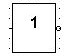
\includegraphics[width=0.1\textwidth,align=t]{../99_Bilder/NOT.jpg}} & \(x_1\) & \(f(x_1)\)\\
			\cline{2-3}
			& 0 & 1\\
			& 1 & 0\\
		\end{tabularx}\\
		\par\noindent
		\textbf{Beschreibung}: Dieses Schaltelement negiert/invertiert das Eingangssignal.
		\subsubsection{OR}
		\begin{tabularx}{0.48\textwidth}{lll|l}
			& \(x_1\) & \(x_2\)& \(f(x_1;x_2)\)\\
			\cline{2-4}
			\multirow{3}{*}{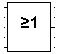
\includegraphics[width=0.1\textwidth,align=t]{../99_Bilder/OR.jpg}} & 0 & 0 & 0\\
			& 0 & 1 & 1\\
			& 1 & 0 & 1\\
			& 1 & 1 & 1\\
		\end{tabularx}\\
		\par\noindent
		\textbf{Beschreibung}: Das Ausgangssignal dieses Schaltsymbol ist genau dann \(1\), wenn \underline{eines} oder \underline{beide} der Eingangssignale \(1\) sind.
		\subsubsection{AND}
		\begin{tabularx}{0.48\textwidth}{lll|l}
			& \(x_1\) & \(x_2\)& \(f(x_1;x_2)\)\\
			\cline{2-4}
			\multirow{3}{*}{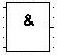
\includegraphics[width=0.1\textwidth,align=t]{../99_Bilder/AND.jpg}} & 0 & 0 & 0\\
			& 0 & 1 & 0\\
			& 1 & 0 & 0\\
			& 1 & 1 & 1\\
		\end{tabularx}\\
		\par\noindent
		\textbf{Beschreibung}: Das Ausgangssignal dieses Schaltsymbol ist genau dann \(1\), wenn \underline{beide} der Eingangssignale \(1\) sind.
		\section{Schaltalgebra}
		Die Schaltalgebra ist ein Spezialfall der booleschen Algebra. In ihr werden alle allgemeinen Aussagen wir \glqq{}wahr\grqq{} und \glqq{}falsch\grqq{} durch Kontaktzustände (also Kontakt geschlossen oder Kontakt offen) ersetzt.\\
		So ist es dann möglich, Schaltnetze durch boolesche Gleichungen zu beschreiben. In der Schaltalgebra ist es zudem üblich, die UND-Funktion als Multiplikationszeichen (\(\cdot\)) und die ODER-Funktion als Pluszeichen (\(+\))darzustellen. Die NICHT-Funktion wird im allgemeinen als Querstrich (\(\bar{x}\)) über der Zustandsvariablen oder durch das mathematische Nicht-Zeichen (\(\neg\)) markiert.\\
		\par\noindent
		Wir schauen uns die folgende \glqq{}logische Gleichung\grqq{} an:\[(E_1 + E_2)\cdot(E_3+E_4) = A_1\]
		Lesen kann man das Ganze dann als:\\
		\textit{(\(E_1\) \textbf{ODER} \(E_2\)) \textbf{UND} (\(E_3\) \textbf{ODER} \(E_4\)) = \(A_1\)}
		\subsection*{Anwendung für die boolesche Logik}
		Generell kann die boolesche Logik bei den meisten Logikproblemen angewendet werden, bei denen die Eingangsvariablen jeweils nur zwei Zustände haben.\\
		Betrachten wir das folgende Beispiel:\\
		Ein Raum hat zwei Türen und ein Fenster. Der angeschlossene Warnmelder soll einen Warnton abgeben, wenn beide Türen mit einem Sicherheitsschloss abgeschlossen sind und entweder ein Bewegungsmelder im Raum oder ein Berührungssensor am Fenster anspringt.\\
		\rule{0.48\textwidth}{0.1pt}\\
		\textit{Wie gehen wir vor, um die Schaltung aufzustellen?}\\
		\par\noindent
		Als Eingangssignale haben wir die beiden Türen \(T_1, T_2\) (UND), sowie den Bewegungsmelder \(B_1\) und den Berührungssensor \(B_2\) (ODER).\\
		Die Türschlösser und die externen Sensoren (UND) lösen zusammen den Warnton aus. Das Ausgangssignal ist der Warnton \(W_1\). So ergibt sich dann die folgende Funktionsgleichung \[W_1 = (E_1\cdot{}E_2)\cdot{}(B_1 + B_2)\]
		Die Funktionalität lässt sich dann mit Hilfe der Gleichung in einer Simulationssoftware\footnote{Zum Beispiel LogicSim.} umsetzten.\\
		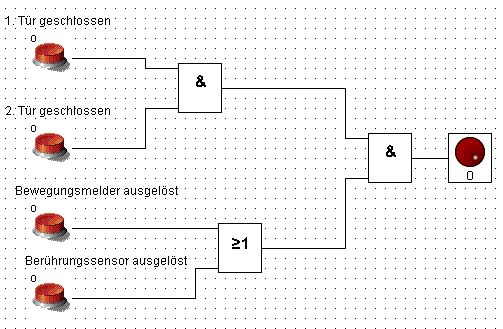
\includegraphics[width=0.48\textwidth]{../99_Bilder/SkrAlarmanlage.jpg}\\
		\section{Schaltungen aufbauen}
		Jetzt haben wir die \textit{boolesche Algebra} und die \textit{Schaltalgebra} kennengelernt. Stellt sich jetzt die Frage: \textit{Wie kann ich das alles anwenden?}\\
		\par\noindent
		\subsection*{Von der Anforderung zur Schaltung}
		In der zuvor dargestellten Beschreibung ging das Aufstellen der Gleichung direkt aus dem Text. Dies ist aber nicht immer der Fall. Daher wollen wir das Vorgehen näher betrachten:\\
		\underline{\textbf{Beispiel:}} Die Primzahl-Maschine kann die Zahlen \(0 - 7\) verarbeiten. Dabei soll die LED besagter Maschine nur dann aufleuchten, wenn die \grq{}gefütterte\grq{} Zahl eine Primzahl ist.\\
		\par\noindent
		\texttt{Wie realisieren wir die Schaltung, die die Primzahl-Maschine repräsentiert?}\\
		\par
		(I) Zunächst müssen wir überlegen, \textbf{wie viele Eingangsvariablen benötigen wir?}\\
		Im Fall der Primzahl-Maschine können wir die Zahlen \(0 - 7\) darstellen, also benötigen wir \(3\) Bit \(\hat{=}\) \(3\) Eingangsvariablen.\\
		\par
		(II) \textbf{Wie viele Ausgangsvariablen benötigt unsere Schaltung?}\\
		Da wir lediglich \underline{eine} LED haben, die leuchtet oder eben nicht, benötigen wir auch nur \textbf{eine} Ausgangsvariable.\\
		\par
		(III) Als nächstes müssen wir herausfinden, \textbf{bei welcher Variablenbelegung (\textit{Eingangsvariablen}) ist unser \textit{Ausgangssignal} 1?}\\
		Für unser Beispiel erstellen wir eine Wahrheitstabelle und tragen in den entsprechenden Stellen eine \(1\) ein.\\
		\par\noindent
		\begin{tabularx}{0.48\textwidth}{|M|M|M|M|}
			\hline
			\rowcolor{codegray!10} \(x_2\) & \(x_1\) & \(x_0\) & \(LED\) \\
			\hline
			0 & 0 & 0 & 0\\
			\hline
			0 & 0 & 1 & 0\\
			\hline
			\rowcolor{green!10} 0 & 1 & 0 & 1\\
			\hline
			\rowcolor{green!10} 0 & 1 & 1 & 1\\
			\hline
			1 & 0 & 0 & 0\\
			\hline
			\rowcolor{green!10} 1 & 0 & 1 & 1\\
			\hline
			1 & 1 & 0 & 0\\
			\hline
			\rowcolor{green!10} 1 & 1 & 1 & 1\\
			\hline
		\end{tabularx}\\
		\par
		(IV) Aus der Tabelle, schreiben wir die \textbf{Variablenbelegungen jeweils als Konjunktion} (UND-Verknüpfung).\\
		Für die obige Tabelle ergibt sich somit:
		\begin{align*}
			LED_2 = \overline{x_2} \cdot{} x_1 \cdot{} \overline{x_0}\\
			LED_3 = \overline{x_2} \cdot{} x_1 \cdot{} x_0\\
			LED_5 = x_2 \cdot{} \overline{x_1} \cdot{} x_0\\
			LED_7 = x_2 \cdot{} x_1 \cdot{} x_0\\
		\end{align*}
		\indent
		(V) Aus dieser Auflistung \textbf{stellen wir die Gleichung auf}, die Grundlage für die Schaltung ist.
		\begin{align*}
			LED & = LED_2 + LED_3 + LED_5 + LED_7\\
			& = (\overline{x_2} \cdot{} x_1 \cdot{} \overline{x_0}) + (\overline{x_2} \cdot{} x_1 \cdot{} x_0) +\\
			& (x_2 \cdot{} \overline{x_1} \cdot{} x_0) + (x_2 \cdot{} x_1 \cdot{} x_0)
		\end{align*}
		\par
		(VI) Unter Verwendung der Gleichung \textbf{realisieren wir die Schaltung in der Simulationssoftware\footnote{LogicSim}}.\\
		\par\noindent
		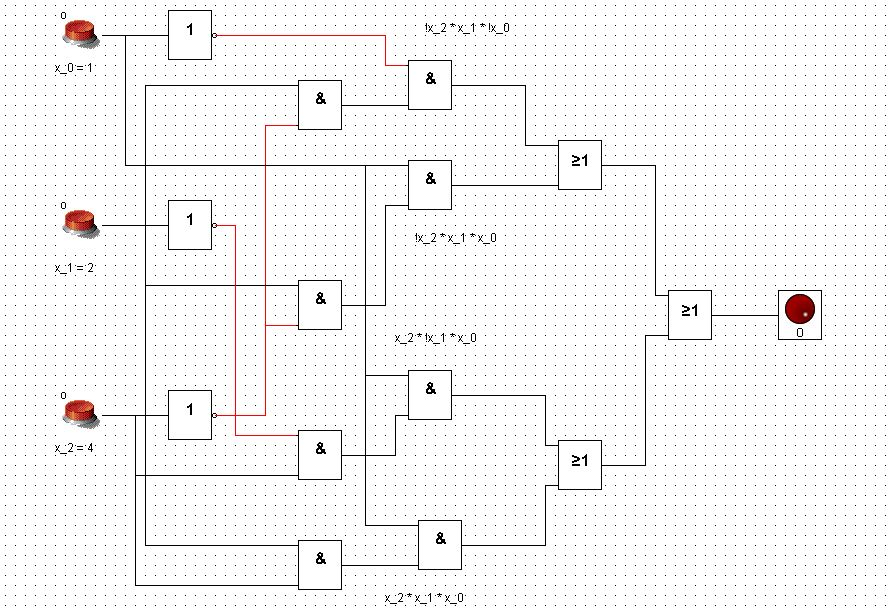
\includegraphics[width=0.48\textwidth]{../99_Bilder/prim.jpg}\\
		\par\noindent
		\texttt{\underline{\textbf{Die Vorgehensweise im Überblick}}}
		\begin{itemize}
			\item[(I)] Anzahl der Eingangsvariablen bestimmen
			\item[(II)] Anzahl der Ausgangsvariablen bestimmen
			\item[(III)] Wertetabelle anlegen und füllen
			\item[(IV)] Konjunktionen der \(1\)-Zeilen aufstellen
			\item[(V)] Gleichung aufstellen (ODER-Verknüpfung der Konjunktionen)
			\item[(VI)] Schaltung realisieren		
		\end{itemize}
	\end{worksheet}
\end{document}